\documentclass[conference]{IEEEtran}

\usepackage{cite}
\usepackage{amsmath,amssymb,amsfonts}
\usepackage{graphicx}
\usepackage{booktabs}
\usepackage{textcomp}
\usepackage{url}
\usepackage{balance}
\usepackage[hidelinks]{hyperref}

\graphicspath{{../results/}}

\hypersetup{
  pdftitle={Design and Simulation of a 6-Bit X-Band CMOS Phase Shifter in a 180-nm CMOS Process},
  pdfauthor={Lam Thanh Dat},
  pdfsubject={Technical report on a 6-bit X-band CMOS phase shifter},
  pdfkeywords={CMOS phase shifter, X-band, S-parameters, phased array, 180-nm CMOS}
}

\begin{document}

\title{Design and Simulation of a 6-Bit X-Band CMOS Phase Shifter in a 180-nm CMOS Process}

\author{
\IEEEauthorblockN{Lam Thanh Dat}
\IEEEauthorblockA{
\textit{Department of Telecommunications, Faculty of Electrical and Electronics Engineering}\\
\textit{Ho Chi Minh City University of Technology (HCMUT), VNU-HCM}\\
Ho Chi Minh City, Vietnam
}
}

\maketitle

\begin{abstract}
This paper documents the design and reproducible postprocessing of a 6-bit
digital phase shifter for X-band operation in a TSMC 180-nm CMOS design
environment. Six binary-weighted cells with nominal increments of 5.625,
11.25, 22.5, 45, 90, and 180 degrees are cascaded to provide 64 control
states. The circuit combines switched low-pass, band-pass, and high-pass
networks synthesized for a 10-GHz center frequency and a 50-ohm system.
Historically reported NMOS samples give an equivalent on-state resistance and
off-state capacitance of approximately 3.33 ohms and 57.8 fF at 10 GHz,
respectively; the native device-characterization export is unavailable.
Preserved Cadence S-parameter exports are independently processed for all
64 states at 9, 10, and 11 GHz. The offset-removed phase-error
root-mean-square value is 2.28 degrees at 10 GHz and 3.67 degrees over all
192 state-frequency samples. Across the aggregate data, the mean insertion
loss is 15.69 dB with 1.73 dB variation, while the mean and minimum input
return losses are 9.49 and 5.48 dB, respectively. The results confirm accurate
digital phase progression but identify transmission loss and impedance
matching as the dominant limitations. The artifact includes the preserved
OpenAccess schematic source and top-level layout and reproduces the numerical
analysis, but not the original Cadence simulation environment, post-layout
verification, or measured performance.
\end{abstract}

\begin{IEEEkeywords}
CMOS phase shifter, digital phase shifter, X-band, S-parameters, phased
array, 180-nm CMOS.
\end{IEEEkeywords}

\section{Introduction}

Digitally stepped phase shifters are key radio-frequency (RF) blocks in
phased-array transmit/receive modules because they set the relative phase at
each antenna element and therefore control the array beam direction. A
6-bit architecture provides 64 discrete phase states and a nominal least
significant bit (LSB) of 5.625 degrees. Switched high-pass/low-pass and
related filter networks are established passive implementations for X-band
phase control \cite{wang2015,xiong2017}. CMOS integration can simplify
digital control and reduce static power, but the finite switch resistance,
off-state capacitance, substrate loss, and limited passive-element quality
factor make low-loss operation difficult at 8--12 GHz
\cite{alsuraisry2015,kang2009}.

This work documents a 6-bit X-band design centered at 10 GHz and evaluates
its complete 64-state response. The technical objectives are fourfold:
describe the binary-weighted circuit architecture, quantify the switch
nonidealities used in design tuning, define a reproducible data-reduction
method, and separate demonstrated simulation results from unverified
physical-design claims. Particular attention is given to phase-error
definitions because a common frequency-dependent phase offset can otherwise
be confused with state-dependent phase nonlinearity.

\section{Circuit Design}

\subsection{Digital Phase Coding}

Let $b_k\in\{0,1\}$ denote the control of phase bit $k$, with $k=0$ for the
5.625-degree LSB and $k=5$ for the 180-degree most significant bit. The ideal
relative phase of state $i$ is
\begin{equation}
  \phi_{i,\mathrm{ideal}}
  = 5.625^\circ\sum_{k=0}^{5} 2^k b_k,
  \qquad i=\sum_{k=0}^{5}2^k b_k .
  \label{eq:phase_code}
\end{equation}
Thus, the 64 codes cover 0 to 354.375 degrees in 5.625-degree increments.
Each cell switches between a reference path and a phase-shifting path. The
six cells are cascaded between 50-ohm ports, as shown in
Fig.~\ref{fig:architecture}. Gate controls use nominal levels of 0 and 1.8 V,
and large gate resistors isolate the RF path from the control source.

\begin{figure*}[!t]
\centering
\scriptsize
\setlength{\tabcolsep}{2.0pt}
\begin{tabular}{c c c c c c c c c c c c c c c}
RF in & $\rightarrow$ &
\fbox{\parbox[c][0.42in][c]{0.68in}{\centering $5.625^\circ$\\cell}} &
$\rightarrow$ &
\fbox{\parbox[c][0.42in][c]{0.68in}{\centering $11.25^\circ$\\cell}} &
$\rightarrow$ &
\fbox{\parbox[c][0.42in][c]{0.68in}{\centering $22.5^\circ$\\cell}} &
$\rightarrow$ &
\fbox{\parbox[c][0.42in][c]{0.68in}{\centering $45^\circ$\\cell}} &
$\rightarrow$ &
\fbox{\parbox[c][0.42in][c]{0.68in}{\centering $90^\circ$\\cell}} &
$\rightarrow$ &
\fbox{\parbox[c][0.42in][c]{0.68in}{\centering $180^\circ$\\cell}} &
$\rightarrow$ & RF out
\end{tabular}
\caption{Functional architecture of the cascaded 6-bit phase shifter. Each
binary control selects the reference or phase-shifting path of one cell.}
\label{fig:architecture}
\end{figure*}

\subsection{NMOS Switch Characterization}

The switch model uses an NMOS with channel length $L=0.18~\mu\mathrm{m}$,
total gate width $W=64~\mu\mathrm{m}$, and 16 fingers. Its source and drain
are characterized as a two-port network in a 50-ohm environment, the body is
grounded, and the gate is biased through a 20-k$\Omega$ resistor. Equivalent
on-state resistance and off-state capacitance are estimated from converted
two-port parameters as
\begin{equation}
\begin{aligned}
 R_{\mathrm{on}}(f)
   &\approx \operatorname{Re}\{Z_{11}(f)\}\big|_{V_G=1.8\,\mathrm{V}},\\
 C_{\mathrm{off}}(f)
   &\approx
   \frac{\operatorname{Im}\{Y_{11}(f)\}}
        {2\pi f}\bigg|_{V_G=0\,\mathrm{V}} .
\end{aligned}
\label{eq:switch_parameters}
\end{equation}
The original report lists $R_{\mathrm{on}}$ values of 3.61, 3.33, and
3.11 $\Omega$ at 9, 10, and 11 GHz, respectively. At 10 GHz,
$\operatorname{Im}\{Y_{11}\}=3.6317$ mS gives
$C_{\mathrm{off}}\approx57.8$ fF and an off-state reactance magnitude of
approximately 275 $\Omega$. The three reported $Z_{11}$ and $Y_{11}$ samples
are transcribed in the repository, and their arithmetic is reproducible.
However, the native NMOS sweep, simulator state, process corner, and PDK
revision are unavailable, so the underlying device simulation is not
reproducible. The reported parasitics are not negligible relative to the
intended lumped elements, particularly for the small phase bits.

\subsection{Phase-Cell Synthesis}

The 5.625-, 11.25-, and 22.5-degree cells use switched low-pass/band-pass
T-networks. The 45- and 90-degree cells use bridged-T variants selected to
reduce the difference in phase slope between the two paths. The 180-degree
cell uses switched high-pass and low-pass paths that produce approximately
opposite 90-degree phase contributions. These architectures follow the
general filter-based approach used in prior X-band digital phase shifters
\cite{wang2015,xiong2017}.

For a phase increment $\Delta\phi$, center angular frequency
$\omega_0=2\pi f_0$, and reference impedance $Z_0$, the ideal starting values
for the small-bit low-pass/band-pass synthesis are
\begin{equation}
\begin{aligned}
 L_1 &= \frac{2Z_0}{\omega_0}\tan\left(\frac{\Delta\phi}{2}\right),&
 C_1 &= \frac{1}{2\omega_0Z_0\tan(\Delta\phi/2)},\\
 L_2 &= \frac{Z_0}{\omega_0}\tan\left(\frac{\Delta\phi}{2}\right),&
 C_2 &= \frac{\sin(\Delta\phi)}{\omega_0Z_0}.
\end{aligned}
\label{eq:small_bit_synthesis}
\end{equation}
Table~\ref{tab:start_values} lists the first-order values obtained at
$f_0=10$ GHz and $Z_0=50~\Omega$. A companion Python calculator regenerates
these values and a machine-readable result table. They are analytical starting
points, not a claim that the final included schematic retains every value
unchanged. Practical tuning compensates for $R_{\mathrm{on}}$,
$C_{\mathrm{off}}$, finite inductor quality factor, and loading between
cascaded cells.

\begin{table}[!t]
\caption{First-Order Ideal Synthesis Values at 10 GHz}
\label{tab:start_values}
\centering
\scriptsize
\setlength{\tabcolsep}{2.0pt}
\begin{tabular}{@{}cl@{}}
\toprule
Phase bit & Analytical starting values\\
\midrule
$5.625^\circ$ &
$L_1=78.19$ pH, $C_1=3.240$ pF; $L_2=39.09$ pH, $C_2=31.20$ fF\\
$11.25^\circ$ &
$L_1=156.8$ pH, $C_1=1.616$ pF; $L_2=78.38$ pH, $C_2=62.10$ fF\\
$22.5^\circ$ &
$L_1=316.6$ pH, $C_1=0.800$ pF; $L_2=158.3$ pH, $C_2=121.8$ fF\\
$45^\circ$ &
$L_1=329.6$ pH, $L_2=960.6$ pH; $C_{\mathrm{off2}}=225.1$ fF,
$C_{\mathrm{off3}}=263.7$ fF\\
$90^\circ$ &
$L_1=795.8$ pH, $L_2=397.9$ pH; $C_{\mathrm{off2}}=318.3$ fF,
$C_{\mathrm{off3}}=636.6$ fF\\
$180^\circ$ &
$L_{\mathrm{LP}}=L_{\mathrm{HP}}=0.7958$ nH;
$C_{\mathrm{LP}}=C_{\mathrm{HP}}=0.3183$ pF\\
\bottomrule
\end{tabular}
\end{table}

The 5.625-degree cell illustrates the parasitic sensitivity. Its ideal
$C_2$ is only 31.2 fF, whereas the characterized switch
$C_{\mathrm{off}}$ is approximately 57.8 fF. Consequently, the switch
capacitance is larger than the ideal phase-setting capacitance, so direct
application of \eqref{eq:small_bit_synthesis} cannot preserve both phase and
matching without circuit-level retuning.

\section{Simulation Data and Metrics}

\subsection{Data Acquisition and Integrity}

Preserved Cadence exports provide transmission phase, transmission magnitude in
decibels, and input reflection magnitude in decibels for every control code
at 9, 10, and 11 GHz. The analysis verifies exactly 64 unique states,
identical controls across the three files, control voltages restricted to
0 or 1.8 V, and the complete state set $i=0,\ldots,63$. The resulting tidy
data set contains 192 state-frequency observations. SHA-256 hashes and a Git
attribute that disables text normalization protect the raw CSV bytes.

The native CSV exports are treated as authoritative. An audit of the
submitted insertion-loss workbook found that its derived 11-GHz column
referenced the 10-GHz source column and then repeated that value in the
average. The affected workbook is therefore excluded from the reproducible
workflow. Recalculation from the native CSV data gives an aggregate mean
insertion loss of 15.69 dB rather than the approximately 15.90-dB workbook
result.

\subsection{Phase Error}

Let $\mathcal{W}(\cdot)$ wrap an angle to
$[-180^\circ,180^\circ)$. The simulated phase of each state is first
referenced to state 0 at the same frequency:
\begin{equation}
\begin{aligned}
 \theta_i(f)
  &=\mathcal{W}\!\left(\angle S_{21,i}(f)-\angle S_{21,0}(f)\right),\\
 e_i(f)
  &=\mathcal{W}\!\left(\theta_i(f)-\phi_{i,\mathrm{ideal}}\right).
\end{aligned}
\label{eq:phase_error}
\end{equation}
For $N=64$ states, the common phase offset and offset-removed phase-error
root-mean-square (RMS) value are
\begin{equation}
\begin{aligned}
 \bar e(f) &= \frac{1}{N}\sum_{i=0}^{N-1}e_i(f),\\
 \sigma_\phi(f) &=
 \sqrt{\frac{1}{N}\sum_{i=0}^{N-1}\left[e_i(f)-\bar e(f)\right]^2}.
\end{aligned}
\label{eq:phase_rms}
\end{equation}
The total RMS,
$\sqrt{N^{-1}\sum_i e_i^2}$, is also reported so that the common offset is
not hidden. Aggregate values apply the same population definitions to all
192 observations.

\subsection{Amplitude and Matching}

Insertion loss (IL) and input return loss (RL) are derived directly from the
simulated scattering parameters:
\begin{equation}
  IL_i(f)=-S_{21,i,\mathrm{dB}}(f),\qquad
  RL_i(f)=-S_{11,i,\mathrm{dB}}(f).
\label{eq:loss_metrics}
\end{equation}
Their state variations are population standard deviations about the
corresponding mean. Minimum RL is included because a mean value alone can
conceal poorly matched control states.

\begin{table*}[!t]
\caption{Recalculated 64-State S-Parameter Statistics}
\label{tab:results}
\centering
\scriptsize
\setlength{\tabcolsep}{3.4pt}
\begin{tabular}{@{}c ccc ccc ccc@{}}
\toprule
 & \multicolumn{3}{c}{Phase error (deg)} &
 \multicolumn{3}{c}{Insertion loss (dB)} &
 \multicolumn{3}{c}{Input return loss (dB)}\\
\cmidrule(lr){2-4}\cmidrule(lr){5-7}\cmidrule(l){8-10}
$f$ & Mean & Offset-removed RMS & Total RMS &
Mean & RMS variation & Min.--max. &
Mean & RMS variation & Minimum\\
\midrule
9 GHz  & $-5.03$ & 3.92 & 6.37 & 16.26 & 1.91 & 12.92--20.62 & 10.88 & 3.44 & 5.92\\
10 GHz & $-2.17$ & 2.28 & 3.15 & 15.72 & 1.66 & 12.77--19.48 &  9.46 & 2.30 & 5.78\\
11 GHz & $+0.89$ & 1.55 & 1.79 & 15.08 & 1.37 & 12.59--18.07 &  8.14 & 1.70 & 5.48\\
Aggregate & $-2.10$ & 3.67 & 4.23 & 15.69 & 1.73 & 12.59--20.62 & 9.49 & 2.81 & 5.48\\
\bottomrule
\end{tabular}
\end{table*}

\begin{figure*}[!t]
\centering
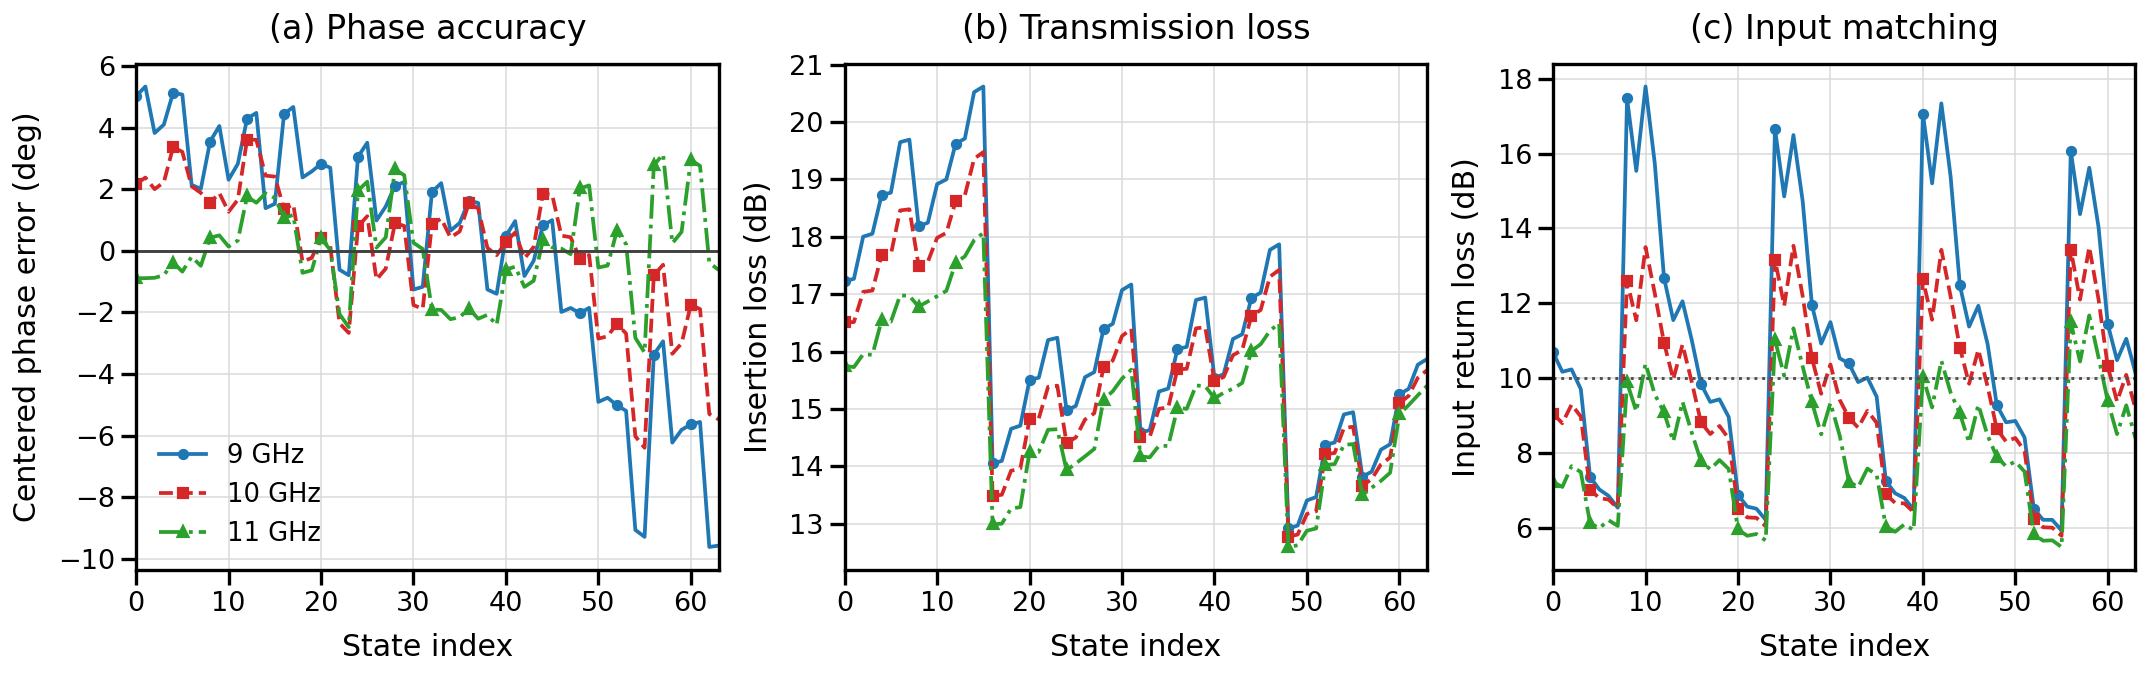
\includegraphics[width=\textwidth]{phase_shifter_performance_overview.png}
\caption{Statewise simulation results at 9, 10, and 11 GHz:
(a) phase error after subtracting the mean error at each frequency,
(b) insertion loss, and (c) input return loss. The dotted horizontal line in
panel (c) marks 10 dB.}
\label{fig:state_metrics}
\end{figure*}

\section{Results}

\subsection{Phase Accuracy}

At 10 GHz, the common phase offset is $-2.17^\circ$ and the state-dependent
RMS error after removing this offset is $2.28^\circ$. The corresponding total
RMS is $3.15^\circ$, demonstrating why the offset definition must be stated.
The offset-removed RMS decreases from $3.92^\circ$ at 9 GHz to
$1.55^\circ$ at 11 GHz, while the mean error changes from
$-5.03^\circ$ to $+0.89^\circ$. Therefore, state linearity improves toward
11 GHz even though the common phase bias shifts with frequency.

Across all 192 observations, the global offset-removed RMS is
$3.67^\circ$. This aggregate value includes both state-dependent dispersion
and the variation of the frequency-specific mean errors. It should not be
interpreted as a continuous-band metric because only three discrete frequency
points are available.

\subsection{Insertion Loss}

Mean IL decreases monotonically from 16.26 dB at 9 GHz to 15.08 dB at
11 GHz. The state variation likewise decreases from 1.91 to 1.37 dB.
Nevertheless, the absolute loss remains high at every sampled frequency. State
15, corresponding to an ideal phase of 84.375 degrees, produces the maximum
IL at all three frequencies: 20.62, 19.48, and 18.07 dB at 9, 10, and
11 GHz, respectively. This persistent extreme indicates a systematic
code-dependent loss mechanism rather than random numerical scatter.

The 15.72-dB mean IL obtained at 10 GHz is close in magnitude to the
15.7-dB typical loss reported for a fabricated 0.18-$\mu$m CMOS 6-bit
X-band design at 9.5 GHz \cite{kang2009}. This numerical similarity is
context only: different circuits, models, de-embedding conditions, and the
absence of confirmed measurements in the present work prevent a direct
performance-equivalence claim.

\subsection{Input Matching}

The average input RL degrades with increasing frequency, from 10.88 dB at
9 GHz to 8.14 dB at 11 GHz. More importantly, the minimum RL is below
6 dB at all three frequencies. State 55, corresponding to an ideal phase of
309.375 degrees, is consistently the least-matched state, with RL values of
5.92, 5.78, and 5.48 dB. Hence, even at 9 GHz, where the average RL exceeds
10 dB, the design does not maintain 10-dB matching over all 64 states.

\section{Critical Assessment}

\subsection{Dominant Technical Tradeoffs}

The simulations demonstrate the intended digital phase progression, but phase
accuracy is obtained at the cost of high loss and uneven input matching. Three
mechanisms are consistent with the available evidence. First,
$R_{\mathrm{on}}$ is in series with the RF path and dissipates power in each
cascaded stage. Second, finite inductor quality factor adds loss and modifies
the ideal network phase. Third, $C_{\mathrm{off}}$ is comparable to, or
larger than, phase-setting capacitances in the small bits, shifting resonance
and disturbing the nominal 50-ohm termination. Cascading six imperfectly
matched cells can then magnify state-dependent reflection and transmission
variation.

These mechanisms are physically plausible, but the available files do not
isolate their individual contributions. In particular, inductor model
revisions, substrate loss, layout coupling, and extraction status are not
documented sufficiently to support a quantitative loss budget.

\subsection{Evidence and Artifact Boundary}

The exact Cadence and simulator versions, TSMC PDK revision, process corner,
temperature, and supply-tolerance conditions are not confirmed. The available
files also do not establish whether the 64-state exports are schematic,
parasitic-extracted, or electromagnetic post-layout simulations. No verified
DRC, LVS, parasitic-extraction, Monte Carlo, chip-area, power-handling, or
measured-hardware results are available. Accordingly, this work should be
described as a circuit-simulation study, not as a tapeout-ready or
experimentally validated integrated circuit.

The public artifact includes the student-created OA schematic source and
top-level layout but excludes the licensed TSMC PDK, device models, rule decks,
and PDK-derived support files. It also lacks the ADE/Assembler/Maestro state,
netlists, and code-sweep definition needed to rerun the original simulations.
The preserved outputs and downstream numerical analysis remain available.

\subsection{Recommended Next Steps}

The highest-priority work is to establish a traceable simulation baseline:
record the PDK and simulator revisions, define process-voltage-temperature
corners, and repeat a dense 8--12-GHz sweep. Post-layout parasitic extraction
and electromagnetic analysis of inductors, interconnect, and coupling should
follow. Circuit optimization should jointly address switch
$R_{\mathrm{on}}C_{\mathrm{off}}$ tradeoffs, passive-element quality factor,
local matching for the worst cells, and cascade ordering. Finally, the
64-state evaluation should be repeated across corners and Monte Carlo samples
before fabrication and measurement.

\section{Conclusion}

\balance

A 6-bit X-band phase shifter with 64 binary-weighted states was designed in a
TSMC 180-nm CMOS environment and evaluated from native Cadence exports at
9, 10, and 11 GHz. The independently recalculated 10-GHz results give a
2.28-degree offset-removed phase-error RMS, 15.72-dB mean insertion loss, and
9.46-dB mean input return loss.
Across all 192 samples, the corresponding
values are 3.67 degrees, 15.69 dB, and 9.49 dB. The phase response is the
strongest aspect of the design; insertion loss, amplitude variation, and
worst-state matching are the principal limitations. Further claims require
dense-frequency, corner, extracted-layout, electromagnetic, and measured
validation.

\section*{Acknowledgment}

The author thanks Dr. Hoang Manh Ha for supervising this academic project at
Ho Chi Minh City University of Technology, VNU-HCM.

\begin{thebibliography}{00}

\bibitem{wang2015}
Q. Wang \textit{et al.}, ``Design of an X-band 6-bit phase shifter,'' in
\textit{Proc. 8th Int. Symp. Comput. Intell. Design (ISCID)}, Hangzhou,
China, 2015, pp. 539--542, doi:
\url{https://doi.org/10.1109/ISCID.2015.108}.

\bibitem{alsuraisry2015}
H. Alsuraisry \textit{et al.}, ``A X-band digitally controlled 5-bit phase
shifter in 0.18-$\mu$m CMOS technology,'' in \textit{Proc. Asia-Pacific
Microw. Conf. (APMC)}, Nanjing, China, 2015, pp. 1--3,
doi: \url{https://doi.org/10.1109/APMC.2015.7413072}.

\bibitem{xiong2017}
Y. Xiong and G. Wang, ``An X-band 6-bits highly-accurate digital-stepped
phase shifter MMIC for phased array system,'' in \textit{Proc. 3rd IEEE Int.
Conf. Comput. Commun. (ICCC)}, Chengdu, China, 2017, pp. 826--829,
doi: \url{https://doi.org/10.1109/CompComm.2017.8322659}.

\bibitem{kang2009}
D.-W. Kang, B.-H. Ku, and S. Hong, ``Design of X-band 6-bit CMOS phase
shifter for phased array T/R modules,'' \textit{Microw. Opt. Technol. Lett.},
vol. 51, no. 10, pp. 2404--2406, Oct. 2009,
doi: \url{https://doi.org/10.1002/mop.24663}.

\end{thebibliography}

\end{document}
